
\documentclass[13pt]{article}
\usepackage[T1]{fontenc}
\usepackage[francais]{babel}
\usepackage{amsmath}

\usepackage[margin=0.75in]{geometry}
\usepackage{courier}
\usepackage{color}
\usepackage{listings}
\usepackage{graphicx}
\setcounter{section}{4}
\setcounter{page}{7}
\begin{document}


\section{Organigrammes des algorithmes des principales m�thodes}

Voici les diff�rents algorithmes (non d�taill�s), ici sous forme d'organigrammes, des m�thodes que nous impl�menterons en Java dans nos classes. Nous avons pens� � mettre les m�thodes d'ajout, de suppression et de mise � jour dans une interface que nos diff�rentes classes (Malade, Docteur, Infirmier) impl�menterons puisque l'on pourra effectuer ces op�rations sur toutes ces classes d'objets.\\

\textbf{Ajout d'un \og objet \fg (Malade, Docteur, Infirmier) dans la base de donn�es}


\begin{figure}[h]
	\centering
		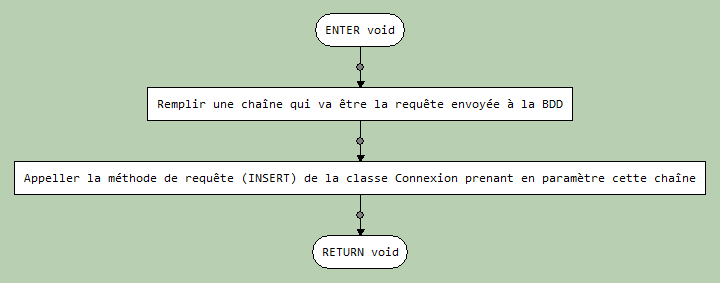
\includegraphics[scale=0.60]{A3}
	\label{fig:A3}
\end{figure}


\textbf{Suppression d'un \og objet \fg de la base de donn�es}

\begin{figure}[h]
	\centering
		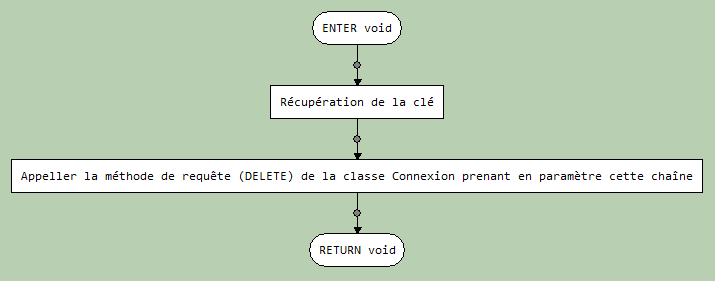
\includegraphics[scale=0.60]{A2}
	\label{fig:A2}
\end{figure}

\textbf{Mise � jour d'un \og objet \fg dans la base de donn�es}

\begin{figure}[h]
	\centering
		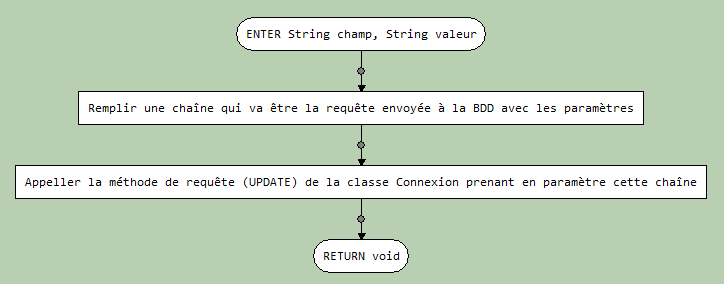
\includegraphics[scale=0.60]{A1}
	\label{fig:A1}
\end{figure}

\newpage
\textbf{Ajout d'une Hospitalisation dans la base de donn�es}

\begin{figure}[h]
	\centering
		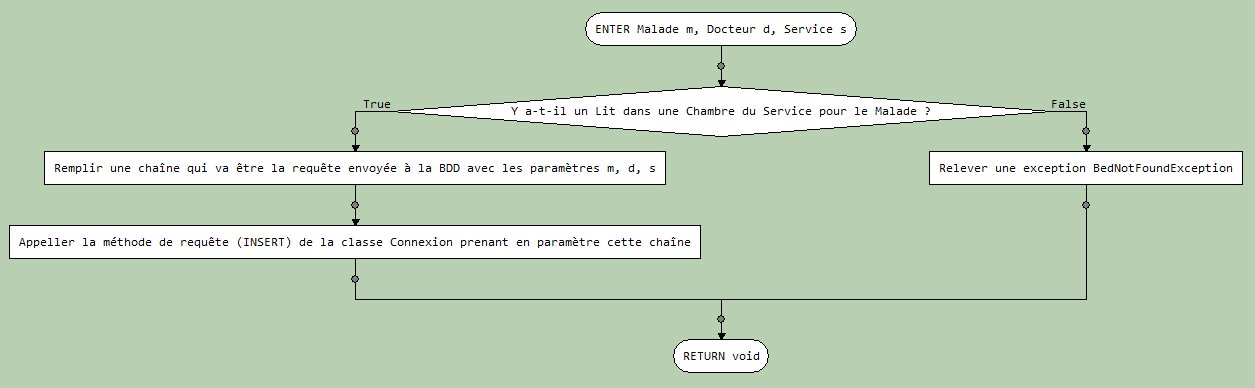
\includegraphics[scale=0.45]{A4}
	\label{fig:A4}
\end{figure}

\textbf{Historisation d'une Hospitalisation dans la base de donn�es}

\begin{figure}[h]
	\centering
		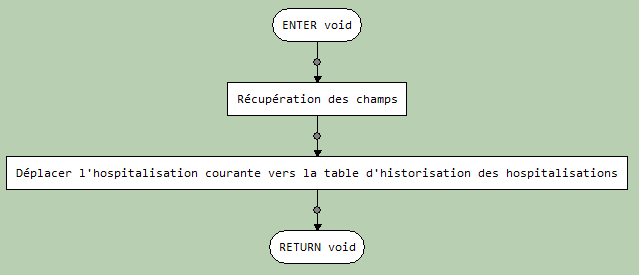
\includegraphics[scale=0.60]{A5}
	\label{fig:A5}
\end{figure}

\section{Conclusion}

 Cette phase de conception nous a permis de bien d�finir notre projet afin de nous r�partir les t�ches de mani�re pr�cise. Nous savons donc maintenant exactement comment nous allons proc�der, et la phase de r�alisation devrait se d�rouler sans probl�me majeur. En effet, nous n'avons normalement rien oubli� et remplit tout les objectifs de ce projet, qui va nous demandez un travail r�gulier et organiser afin de la menez au mieux dans le temps imparti. 

\end{document}